\subsection{Arduino Nano 33 BLE}
\begin{figure}[h!]
	\centering
 	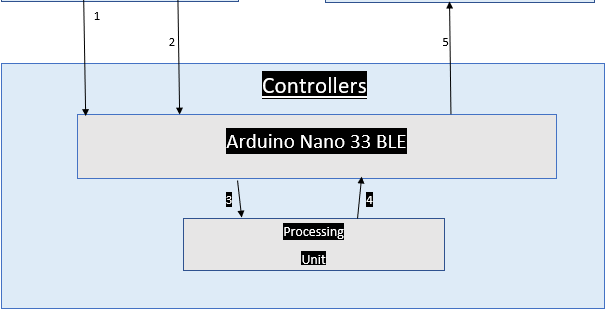
\includegraphics[width=0.60\textwidth]{images/Controller subsystems}
 \caption{Controller Subsystem}
\end{figure}

\subsubsection{Assumptions}
Not applicable.

\subsubsection{Responsibilities}
The main responsibility of Arduino nano is to receive analog signals from temperature sensor and IMU sensors. CPU inside then process analog data then transfers process data to UI/UX layer via Bluetooth.
\\\\
NINA-b3 (nRF52840) chip inside Arduino nano BLE 33 sense handles processing data. Arduino nano will operate at 5-3.3 V powered by 9V battery (9V will be divided with voltage divider) after the completion of Bluetooth Hydrometer.
\\\\
Arduino 1.8.13 is used to program Arduino nano 33 BLE sense which is the proprietary software Arduino provides. Arduino serial monitor will be used to test the results. 

\subsubsection{Subsystem Interfaces}
Data elements will pass through this interface.

\begin {table}[H]
\caption {Subsystem interfaces} 
\begin{center}
    \begin{tabular}{ | p{1cm} | p{6cm} | p{3cm} | p{3cm} |}
    \hline
    ID & Description & Inputs & Outputs \\ \hline
    & Controller interface & \pbox{3cm}{input 1 \\ input 2 \\ input 4} & \pbox{3cm}{output 5}  \\ \hline
    \end{tabular}
\end{center}
\end{table}

\subsection{Processing Unit}
\subsubsection{Assumptions}
Hydrometer is always turned on whenever it's inside the fermentation vessel. Since, position of hydrometer is needed for specific gravity, it's assumed that the hydrometer is floating.

\subsubsection{Responsibilities}
60 MHz CPU is responsible for processing temperature and specific gravity data, that it receives from built-in IMU and temperature sensors. Arduino nano is programmed to handle those data whenever nano is turned on. It outputs the accurate temperature and specific gravity data after processing.

\subsubsection{Processing Unit Interface}

\begin {table}[H]
\caption {Subsystem interfaces} 
\begin{center}
    \begin{tabular}{ | p{1cm} | p{6cm} | p{3cm} | p{3cm} |}
    \hline
    ID & Description & Inputs & Outputs \\ \hline
    & Processing Unit Interface & \pbox{3cm}{input 3} & \pbox{3cm}{output 4}  \\ \hline
    \end{tabular}
\end{center}
\end{table}

\subsection{Bluetooth Interface}
\subsubsection{Assumptions}
Not Applicable.

\subsubsection{Responsibilities}
Bluetooth will be handled by ArduinoBLE library. BLE library provides various functions to send data from Arduino to a Bluetooth device.  Functions needed for Bluetooth Hydrometer are listed below. Functions will be added or removed depending on the modifications required in the future.

\begin{lstlisting}
#include <ArduinoBLE.h>			//Bluetooth library needs to be included
BLE.begin()
-	Returns 1 on success and 0 on failure
BLE.central()				//For connecting Bluetooth devices (central - Bluetooth device)
-	Returns BLEDevice representing the central
BLEService (uuid)
BLEServide(index, uuid)
-	Returns BLEService for provided parameters
-	Index - index of service
-	Uuid - uuid(string)	//BluetoothHydrometer
BLE.read()
-	True, if successful, false on failure
BLE.notify()
-	Notify change in BLECharacteristic //change in temperature or accel and gyro data
BLE.setLocalName(name)
-	Name: local name to be used when advertising
-	Returns: none
BLE.addService(service)
-	Service to add
-	Returns none
BLE.setAdvertisedService(bleService)
-	Returns none
-	BLEService to use UUID from
bleService.addCharacteristic(bleCharacteristic)
-	Add a BLECharacteristic to the BLE service
bleCharacteristic.writeValue(value)
-	Value - value to write
-	bleCharacteristic - temperature and position data for Bluetooth Hydrometer
BLE.advertise()
-	Start advertising
-	Returns 1 on success, 0 on failure
\end{lstlisting}

\subsubsection{Subsystem Interfaces}
\begin {table}[H]
\caption {Subsystem interfaces} 
\begin{center}
    \begin{tabular}{ | p{1cm} | p{6cm} | p{3cm} | p{3cm} |}
    \hline
    ID & Description & Inputs & Outputs \\ \hline
    & Bluetooth Interface & \pbox{3cm}{input 4} & \pbox{3cm}{output 5}  \\ \hline
    \end{tabular}
\end{center}
\end{table}